%% Run LaTeX on this file several times to get Table of Contents,
%% cross-references, and citations.

\documentclass[11pt]{book}
\usepackage{gvv-book}
\usepackage{gvv}
\usepackage[sectionbib,authoryear]{natbib}% for name-date citation comment the below line
\setcounter{secnumdepth}{3}
\setcounter{tocdepth}{2}

\makeindex

\begin{document}

\frontmatter

\booktitle{GEOMETRY}

\subtitle{Through Algebra}

\AuAff{Chakali Suresh}

\titlepage

\tableofcontents

\setcounter{page}{1}

\mainmatter

\chapter{Triangle}
Consider a triangle with vertices
\begin{align}
\vec{A} = \myvec{0 \\ -5},\,
\vec{B} = \myvec{-2 \\ -4},\,
\vec{C} = \myvec{-5 \\ -4}
\end{align}

\section{Vectors}
\begin{enumerate}[label=\thesection.\arabic*.,ref=\thesection.\theenumi]
\numberwithin{equation}{enumi}
\item the direction vector of $AB$ is defined as 
\begin{align}
 \vec{B}-
  \vec{A}
\end{align}
Find the direction vectors of $AB, BC$ and $CA$.
\\
\solution
\begin{enumerate} 
\item  The Direction vector of $AB$ is 
\begin{align}&= \vec{B} - \vec{A} \\
 &= \myvec{ -2  -(0)\\ -4 - (-5) } \\&= \myvec{ -2\\ 1 }
 \end{align}
\item The Direction vector of $BC$ 
\begin{align}&= \vec{C} - \vec{B}\\
 &= \myvec{ -5 - (-2)\\ -4 - (-4) } \\&= \myvec{-3\\ 0 }
  \end{align}
  \item  The Direction vector of $CA$  
  \begin{align} &= \vec{A} - \vec{C} \\ 
 &= \myvec{ 0 - (-5)\\ -5 - (-4) } \\&= \myvec{ 5 \\ -1 }
  \end{align}
 \end{enumerate}

 \item The length of side $AB,BC$ and $AC$ is

		\solution
Given, 
\begin{align}
\vec{A} = \myvec{0\\-5},\\
\vec{B} = \myvec{-2\\-4},\\
\vec{C} = \myvec{-5\\-4} 
\end{align}

Now solving for $AB$,\\
\begin{align}
\norm{\vec{A}-\vec{B}}\ &=  \sqrt{\brak{\vec{A}-\vec{B}}^{\top}\brak{\vec{A}-\vec{B}}} \\
	\vec{A}-\vec{B} &= \myvec{0\\-5} - \myvec{-2\\-4} &= \myvec{2\\-1}\\
\norm{\vec{A}-\vec{B}} &= \sqrt{\myvec{2 & -1}\myvec{2\\-1}}\\
&= \sqrt{\brak{2}^2 +\brak{-1}^2}\\
	\implies \norm{\vec{A}-\vec{B}} &=\sqrt{5}
\end{align}

Now solving for $BC$,\\
\begin{align}
	\norm{\vec{B}-\vec{C}}\ &=  \sqrt{\brak{\vec{B}-\vec{C}}^{\top}\brak{\vec{B}-\vec{C}}} \\
\vec{B}-\vec{C} &= \myvec{3\\0}\\
\norm{\vec{B}-\vec{C}} &= \sqrt{\myvec{3 & 0}\myvec{3\\0}}\\
&= \sqrt{\brak{3}^2+\brak{0}^2}\\
\implies \norm{\vec{B}-\vec{C}} &= \sqrt{9} = 3
\end{align}

Now solving for $AC$,\\
\begin{align}
	\norm{\vec{A}-\vec{C}}\ &=  \sqrt{\brak{\vec{A}-\vec{C}}^{\top}\brak{\vec{A}-\vec{C}}} \\
\vec{A}-\vec{C} &= \myvec{-5\\1}\\
\norm{\vec{A}-\vec{C}} &= \sqrt{\myvec{-5 & 1}\myvec{-5\\1}}\\
&= \sqrt{\brak{-5}^2+\brak{1}^2}\\
\implies \norm{\vec{A}-\vec{C}}&=\sqrt{26}
\end{align}

\item Points $\vec{A}, \vec{B}, \vec{C}$ are defined to be colliner if
	\begin{align}
		\rank{\myvec{1 & 1 & 1 \\ \vec{A} & \vec{B} & \vec{C}}} = 2
	\end{align}
\solution\\
Given that,
\begin{align}
    \vec{A} = \myvec{0\\-5}
    \quad
    \vec{B} &= \myvec{-2\\-4}
    \quad
    \vec{C} = \myvec{-5\\-4}
\end{align}
Given that $\vec{A},\vec{B},\vec{C}$ are collinear if
\begin{align}
    \text{rank}\myvec{
    1 & 1 & 1\\
    \vec{A} & \vec{B} & \vec{C} \\
    } &< 3 
    \label{eq:1.1.3,2}
\end{align} 
Let
\begin{align}
    \vec{R}&=\myvec{
    1 & 1 & 1
    \\
    0 & -2 & -5
    \\
    -5 & -4 & -4
    } 
\end{align} 
The matrix $\vec{R}$ can be row reduced as follows,
\begin{align}
    \label{eq:matthrowoperations}
    \myvec{
    1 & 1 & 1
    \\
    0 & -2 & -5
    \\
    -5 & -4 & -4
    }
	\xleftrightarrow[]{R_3 \leftarrow R_3+(5+R_2)}
    \myvec{
    1 & 1 & 1
    \\
    0 & -2 & -5
    \\
    0 & -1 & -4 
    }
    \\
     \xleftrightarrow[]{R_3\leftarrow -2R_3+R_2}
    \myvec{
    1 & 1 & 1
    \\
    0 & -2 & -5
    \\
    0 & 0 & 3
    }
\end{align}

There are no zero rows. So,
\begin{align}
    \text{rank}\myvec{
    1 & 1 & 1\\
    \vec{A} & \vec{B} & \vec{C} \\
    } &= 3 
\end{align}  
Hence, from \eqref{eq:1.1.3,2} the points $\vec{A},\vec{B},\vec{C}$ are not collinear. 

\begin{figure}[H]
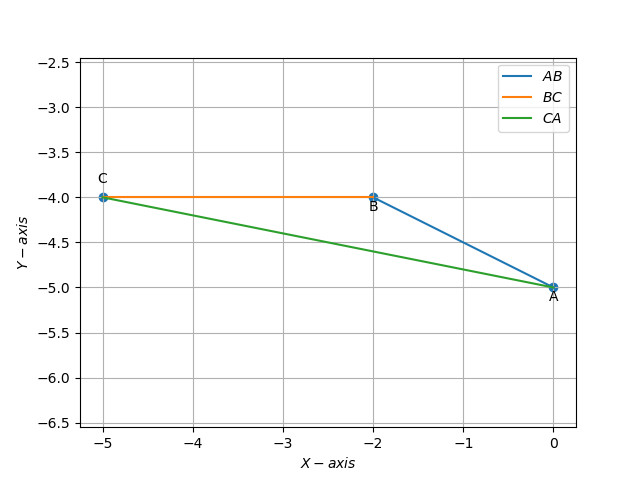
\includegraphics[width=\columnwidth]{/sdcard/Documents/figs/Collinear.png}
\caption{$\vec{A},\vec{B},\vec{C}$ plot}
\label{fig1:Triangle}
\end{figure}

From Fig. \ref{fig1:Triangle}, We can see that $\vec{A},\vec{B},\vec{C}$ are not collinear .

\item The parametric form of the equation of $AB$ is
	\begin{align}
		\vec{x}=\vec{A}+k\vec{m}
	\end{align}
	where\\
	\begin{align}
		\vec{m} = \vec{B} - \vec{A}
	\end{align}
	is the direction vector of $AB$.
	Find the parametric equations of $AB,BC$ and $CA$.

	\solution\\
	The parametric equation for $AB$ is given by
	\begin{align}
		\vec{x} &= \vec{A} + k\vec{m}\\
		\text{where, } \vec{m} &= \vec{B} -\vec{A}\\
		&= \myvec{-2 \\ -4} -\myvec{0\\ -5}\\
		&= \myvec{-2 \\ 1}
	\end{align}
	Hence we get,
	\begin{align}
		\vec{AB}: \vec{x} = &\myvec{0\\-5} + k \myvec{-2\\1}
	\end{align}
	Similarly, 
	\begin{align}
		\vec{BC}: \vec{x} = &\myvec{-2\\-4} + k \myvec{-3\\0}\\
		\vec{CA}: \vec{x} = &\myvec{-5\\-4} + k \myvec{5\\-1}
	\end{align}

\item The normal form of the equation of $\vec{AB}$ is
\begin{align}
\vec{n}^{\top}\myvec{\vec{x}-\vec{A}}=0
\end{align}
where
\begin{align}
\vec{n}^{\top}\vec{m}&=\vec{n}^{\top}\myvec{\vec{B}-\vec{A}}=0
\end{align} 
or,\begin{align}
\vec{n}&=\myvec{0 &1 \\-1 & 0}\vec{m}
\end{align}
then find the normal form of the equations of $\vec{AB}$ $\vec{BC}$ and $\vec{CA}$

\solution:\\
       The normal equation for the side $AB$ is
\begin{align}
\vec{n}^{\top}\myvec{\vec{x}-\vec{A}}&=0\\
\implies
\vec{n}^{\top}\vec{x}&=\vec{n}^{\top}\vec{A}
\end{align}
Now our task is to find the $\vec{n}$ so that we can find $\vec{n}^{\top}$.
As given. 
\begin{align}
  \vec{n} &= \myvec{0 & 1\\
  -1 & 0}\vec{m}
\end{align}
Here $\vec{m} = \vec{B}- \vec{A}$ for side $\vec{AB}$
\begin{align}
\implies
\vec{m}&=\myvec{-2\\-4} - \myvec{0\\-5}\\
&=\myvec{-2\\1}
\end{align}
Now as we have obtained vector $\vec{m}$.we can use this to obtain vector $\vec{n}$
\begin{align}
\vec{n} &= \myvec{0 & 1\\
  -1 & 0}\myvec{-2\\1}
 = \myvec{1\\2}
\end{align}
The transpose of $\vec{n}$ is
\begin{align}
  \vec{n}^{\top}&=\myvec{1 & 2}
\end{align}
Hence the normal equation of side $AB$ is 
\begin{align}
    \myvec{1 & 2}\vec{x}&=\myvec{1 & 2}\myvec{0\\-5}\\
    \implies \myvec{1 & 2}\vec{x} &= -10
\end{align}
\begin{figure}[H]
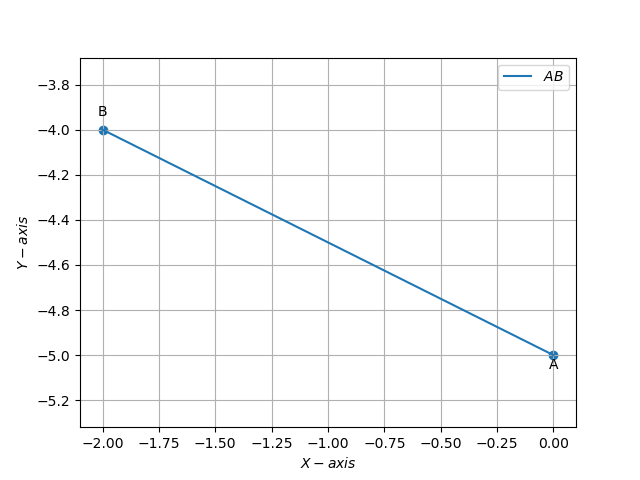
\includegraphics [width=\columnwidth] {/sdcard/Documents/figs/AB.png}
\caption{ The line $\vec{AB}$ plotted}
\label{fig:line AB}
\end{figure}
Similarly
\begin{align}
	\implies
	\vec{BC:} \myvec{0 & 3}\vec{x} &= -12
\end{align}
\begin{figure}[H]
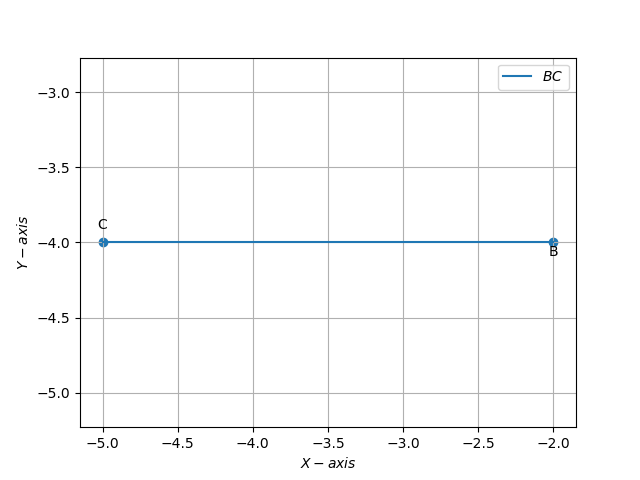
\includegraphics [width=\columnwidth] {/sdcard/Documents/figs/BC.png}
\caption{ The line $\vec{BC}$ plotted}
\label{fig:line BC}
\end{figure}

\begin{align}
	\implies \vec{CA:} \myvec{-1 & -5}\vec{x} &= 25
\end{align}
\begin{figure}[H]
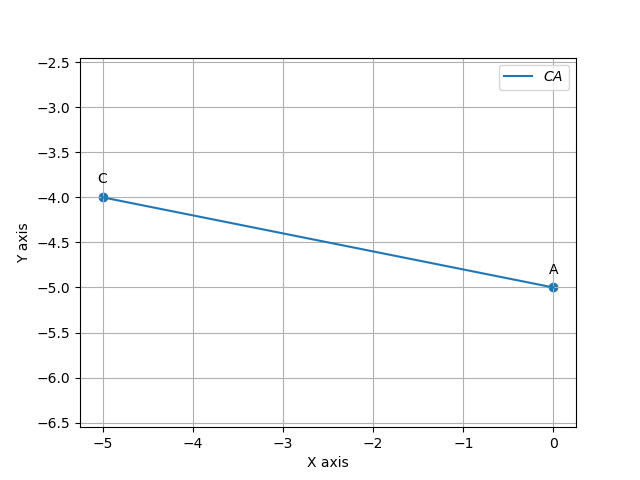
\includegraphics [width=\columnwidth] {/sdcard/Documents/figs/CA.png}
\caption{ The line $\vec{CA}$ plotted}
\label{fig:line CA}
\end{figure}

\item Find the area of the $\triangle ABC$

	\solution\\
Given,
\begin{align}
 \vec{A} = \myvec{0\\-5};
 \vec{B} = \myvec{-2\\-4};
 \vec{C} = \myvec{-5\\-4}
 \end{align}
 \begin{align}
 \vec{A}-\vec{B} &= \myvec{0\\-5} - \myvec{-2\\-4} = \myvec{2\\-1}\\
 \vec{A}-\vec{C} &= \myvec{0\\-5} - \myvec{-5\\-4} = \myvec{5\\-1}\\
\therefore(\vec{A}-\vec{B})\times(\vec{A}-\vec{C}) 
 &= \mydet{2 & -1\\5 & -1}\\
 &= 2 \times -1 - 5 \times (-1)\\ &= -2 + 5\\ &= 3\\
 \implies\frac{1}{2}\norm{(\vec{A}-\vec{B})\times(\vec{A}-\vec{C})} &= \frac{1}{2}\norm{3}= \frac{3}{2}
\end{align}

\item Find the angles $A, B, C$ if 
    \label{prop:angle2d}
  \begin{align}
    \label{eq:angle2d}
   \cos A \triangleq 
\frac{\brak{\vec{B}-\vec{A}}^{\top}{\vec{C}-\vec{A}}}{\norm{\vec{B}-\vec{A}}\norm{\vec{C}-\vec{A}}}
  \end{align}
\solution\\
From the given values of $\vec{A},\vec{B},\vec{C}$,\\
\begin{enumerate}
 \item Finding the value of angle A
\begin{align}
 \vec{B}-\vec{A} &=\myvec{-2\\1}
\end{align}
and 
\begin{align}
 \vec{C}-\vec{A} &= \myvec{-5\\1}
\end{align}
also calculating the values of norms
\begin{align}
 \norm{\vec{B}-\vec{A}} &= \sqrt{5}\\
 \norm{\vec{C}-\vec{A}} &= \sqrt{26}
\end{align}
and by doing matrix multiplication we get,
\begin{align}
\begin{split}
 (\vec{B}-\vec{A})^{\top}(\vec{C}-\vec{A}) &= \myvec{-2&1}\myvec{-5\\1} = 11
\end{split}
\end{align}
So, we get
\begin{align}
 \cos{A} &= \frac{11}{\sqrt{5} \sqrt{26}}\\
 &= \frac{11}{\sqrt{130}}\\
 \implies A& = \cos^{-1}{\frac{11}{\sqrt{130}}}
\end{align}

\item Finding the value of angle B
\begin{align}
 \vec{C}-\vec{B} &=\myvec{-3\\0}
\end{align}
and 
\begin{align}
 \vec{A}-\vec{B} &= \myvec{2\\-1}
\end{align}
also calculating the values of norms
\begin{align}
 \norm{\vec{C}-\vec{B}} &= \sqrt{9} = 3\\
 \norm{\vec{A}-\vec{B}} &= \sqrt{5}
\end{align}
and by doing matrix multiplication we get,
\begin{align}
\begin{split}
 (\vec{C}-\vec{B})^{\top}(\vec{A}-\vec{B}) &= \myvec{-3&0}\myvec{2\\-1} = -6
\end{split}
\end{align}
So, we get 
\begin{align}
	\cos{B} &= \frac{-6}{{3} \sqrt{5}}\\
 &= \frac{-2}{\sqrt{5}}\\
 \implies B& = \cos^{-1}{\frac{-2}{\sqrt{5}}}
\end{align}

\item Finding the value of angle C
\begin{align}
 \vec{A}-\vec{C} &=\myvec{5\\-1}
\end{align}
and 
\begin{align}
 \vec{B}-\vec{C} &= \myvec{3\\0}
\end{align}
also calculating the values of norms
\begin{align}
 \norm{\vec{A}-\vec{C}} &= \sqrt{26}\\
	\norm{\vec{B}-\vec{C}} &= \sqrt{9} = 3
\end{align}
and by doing matrix multiplication we get,
\begin{align}
\begin{split}
 (\vec{A}-\vec{C})^{\top}(\vec{B}-\vec{C}) &= \myvec{5&-1}\myvec{3\\0}\\
 &= 15
\end{split}
\end{align}
so 
\begin{align}
	\cos{C} &= \frac{15}{{3} \sqrt{26}}\\
 &= \frac{5}{\sqrt{26}}\\
 \implies C &= \cos^{-1}{\frac{5}{\sqrt{26}}}
\end{align}
\end{enumerate}

\latexprintindex

\end{enumerate}
\end{document}

 
